\documentclass[10pt]{article}
\usepackage[polish]{babel}
\usepackage[utf8]{inputenc}
\usepackage[T1]{fontenc}
\usepackage{amsmath}
\usepackage{amsfonts}
\usepackage{amssymb}
\usepackage[version=4]{mhchem}
\usepackage{stmaryrd}
\usepackage{graphicx}
\usepackage[export]{adjustbox}
\graphicspath{ {./images/} }

\title{OD SZKOLNIAKA DO ŻAKA }

\author{}
\date{}


\begin{document}
\maketitle
\section*{klasy 5 i 6 szkoły podstawowej \\
 rok szkolny 2022/2023 \\
 Zadania - etap II}
Zadanie 1. Aby dodać trzy ułamki zwykłe (dodatnie, każdy inny) Ania sprowadziła je do najmniejszego wspólnego mianownika równego 15. Po dodaniu ułamków otrzymała wynik 1. Jakie ułamki mogła dodać Ania? Rozważ wszystkie możliwości.

Zadanie 2. Na ramionach kąta \(30^{\circ}\) o wierzchołku \(D\), obrano punkty \(A, B, C\), które są wierzchołkami trójkąta równobocznego o boku długości 2 cm (tak jak na rysunku). Oblicz odległość wierzchołka kąta \(\nless B D A\) od punktu \(A\). Zapisz wszystkie obliczenia.\\
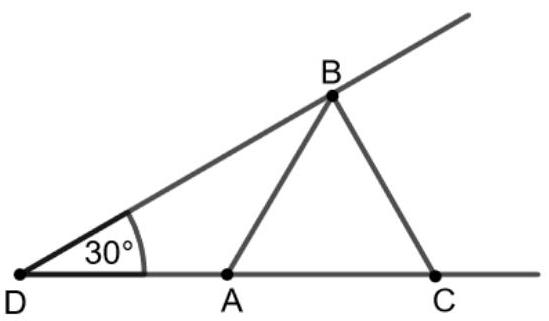
\includegraphics[max width=\textwidth, center]{2024_11_21_2db47e70611255ec3156g-1}

Zadanie 3. Dane są dwie serie liczb tworzonych według pewnych zasad.\\
seria 1: \(1,8,27,64,125, \ldots\)\\
seria 2: \(6,8,10,12,14, \ldots\).\\
Według jakich zasad utworzone są te serie liczb? Ile wynosi iloraz dwunastej liczby w serii 1-szej przez trzydziestą liczbę serii 2-giej?

Zadanie 4. Pewien rolnik posiadał pole uprawne w kształcie prostokąta o wymiarach 120 m na 250 m . Od sąsiada dokupił pas ziemi, zwiększając wymiary swojego pola odpowiednio o 40 m i 20 m . O ile procent zwiększyła się powierzchnia pola uprawnego?

Zadanie 5. Jeżeli na szalce wagi szalkowej położymy czekoladę i odważnik 2 kg , a na drugiej szalce 6 takich samych czekolad i odważnik 50 dag, to waga będzie w równowadze. Ile waży jedna czekolada?


\end{document}